% !TEX program = xelatex
\documentclass[tikz,border=0pt]{standalone}
\usepackage{fontspec,xeCJK,graphicx}
\usetikzlibrary{arrows.meta}
\setmainfont{Times New Roman}
\setCJKmainfont[Path=/Users/april/Library/Fonts/,FontIndex=0,AutoFakeBold=2]{宋体.ttc}
\setCJKfamilyfont{hei}[Path=/Users/april/Library/Fonts/,AutoFakeBold=2]{黑体.ttf}
\newcommand{\hei}{\CJKfamily{hei}}
\begin{document}
\begin{tikzpicture}[x=1cm,y=1cm]
  \node[anchor=north west,inner sep=0] at (0,0)
    {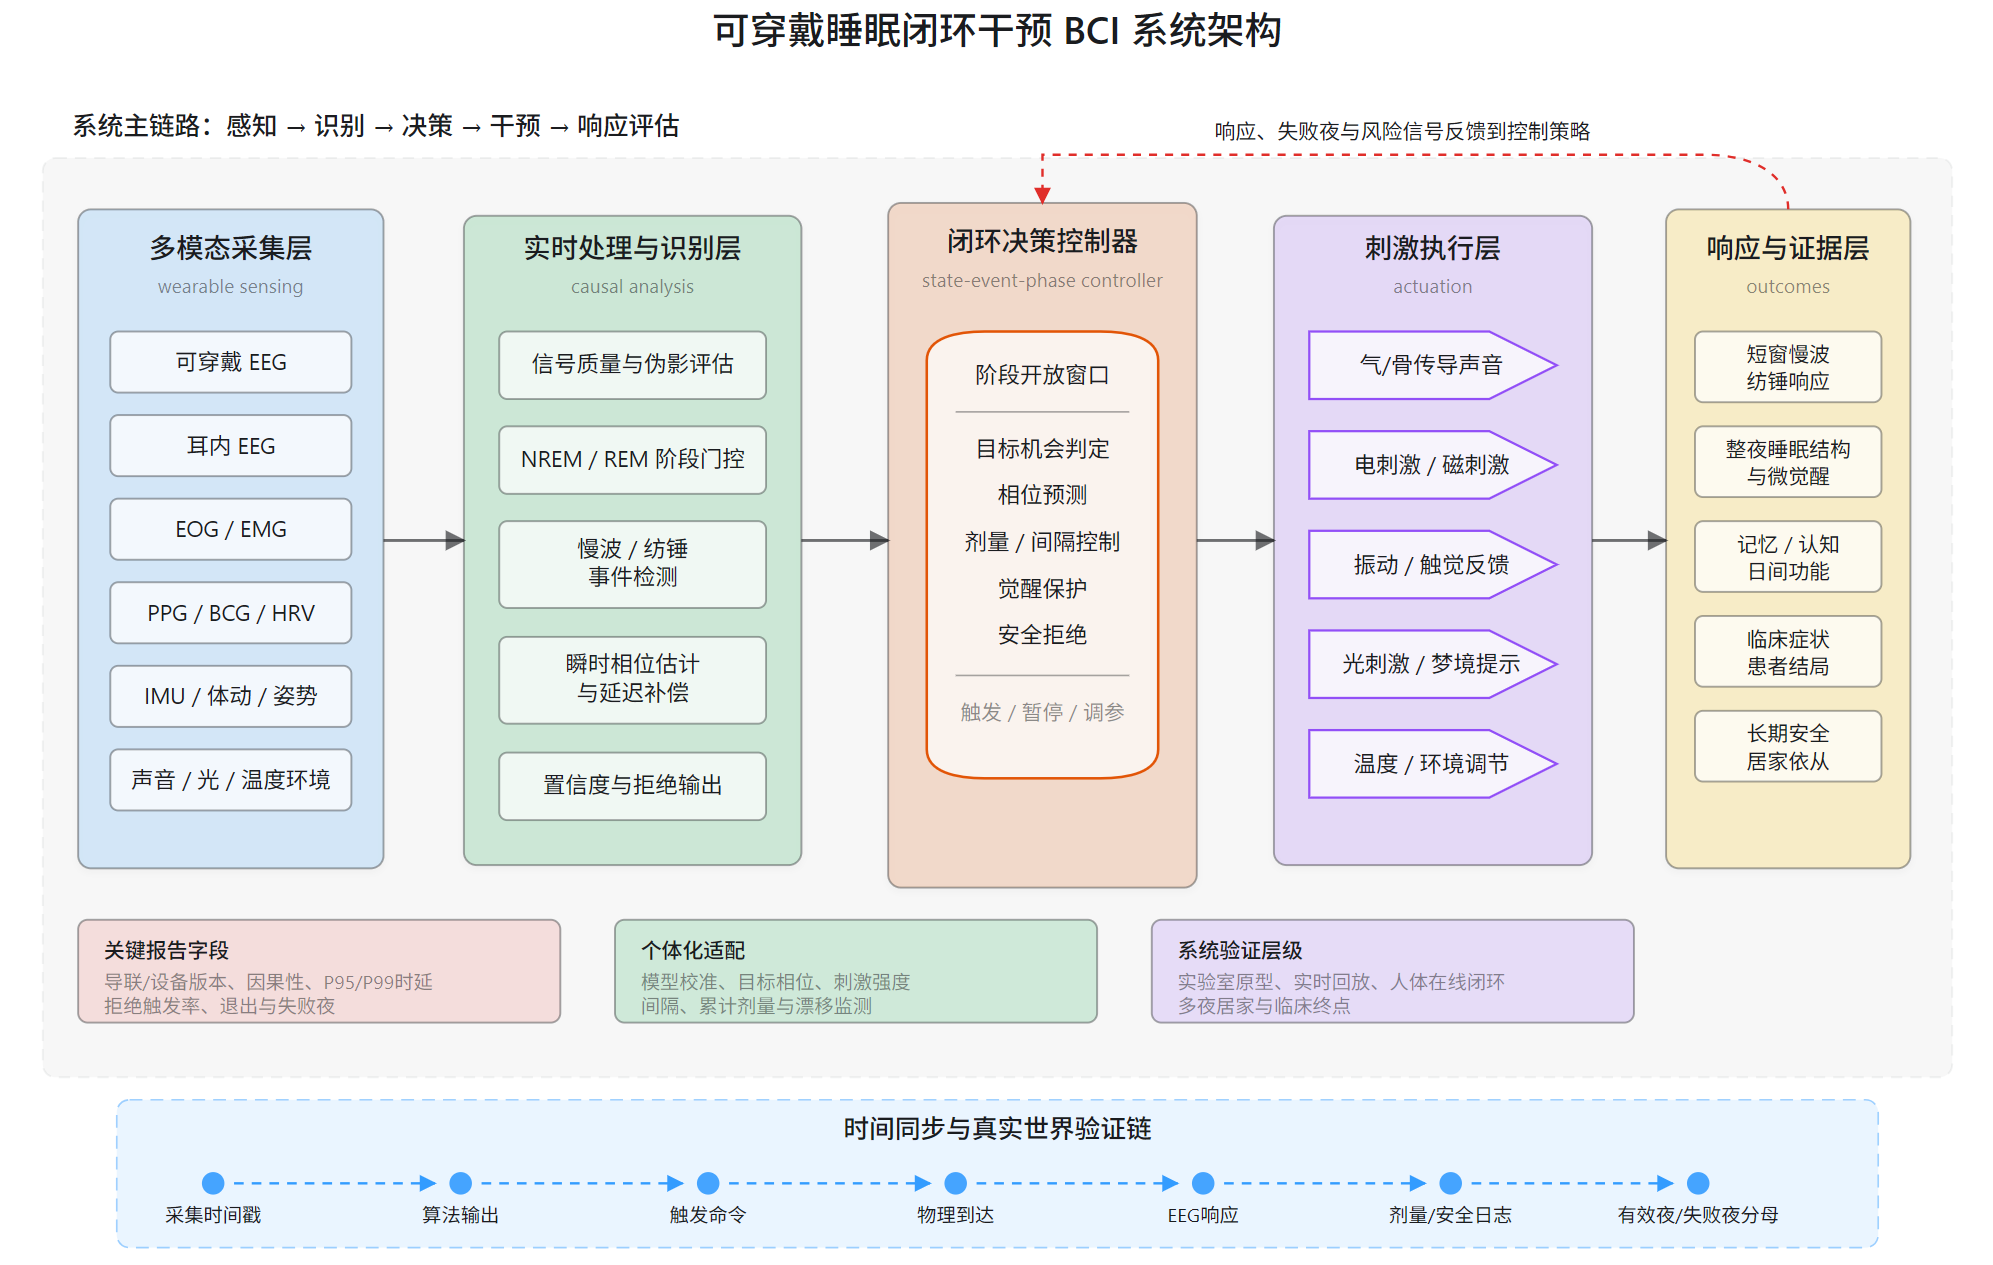
\includegraphics[width=19.93cm]{wearable-sleep-closed-loop-bci-architecture-no-caption.png}};

  \fill[blue!4,rounded corners=0.16cm] (0.42,-12.77) rectangle (19.51,-15.32);
  \draw[blue!35,dashed,rounded corners=0.16cm,line width=0.8pt]
    (0.42,-12.77) rectangle (19.51,-15.32);
  \node[anchor=west,font=\hei\bfseries\fontsize{13}{15}\selectfont]
    at (0.82,-13.10) {控制层级连续谱};
  \node[anchor=east,font=\fontsize{10}{12}\selectfont,text=gray!75]
    at (19.10,-13.10) {实时睡眠信号参与决策的深度逐级增加 $\longrightarrow$};

  \foreach \x/\fillc/\title/\sub in {
    0.80/gray!10/开环刺激/预设时序，无实时信号,
    4.49/blue!8/阶段门控刺激/睡眠阶段决定准入,
    8.18/green!10/事件触发闭环/目标事件逐次触发,
    11.87/orange!12/相位锁定闭环/刺激命中目标相位,
    15.56/red!10/自适应闭环/响应反馈更新参数}
  {
    \fill[\fillc,rounded corners=0.10cm] (\x,-13.42) rectangle +(3.28,-1.48);
    \draw[gray!55,rounded corners=0.10cm,line width=0.65pt]
      (\x,-13.42) rectangle +(3.28,-1.48);
    \node[align=center,font=\hei\bfseries\fontsize{11}{13}\selectfont]
      at (\x+1.64,-13.88) {\title};
    \node[align=center,font=\fontsize{9.2}{11}\selectfont,text=gray!75]
      at (\x+1.64,-14.47) {\sub};
  }
  \foreach \x in {4.28,7.97,11.66,15.35}
    \draw[-{Stealth[length=0.16cm]},blue!60,line width=0.75pt]
      (\x-0.16,-14.16) -- (\x+0.16,-14.16);
\end{tikzpicture}
\end{document}
